\chapter{Experiments and Results}

\section{Retargeting}
In the retargeting phase,  we have successfully transformed two motion clips that enact skills of \textit{hand wave} (Fig \ref{fig:retarget_wave}) and \textit{walk in place} (Fig \ref{fig:retarget_wip}). We were able to retarget these simple motion clips from model in Fig \ref{fig:mocap_hierarchy} to our Nao model (in Fig \ref{fig:nao_hierarchy}). From the below embedded videos, we can clearly observe the smoothness of movements and synchronization with the original clip in term of foot joints, hand and leg movements. 

\begin{figure}[!b]
  \centering
  \href{https://youtu.be/UpT7YPi6Ekc}{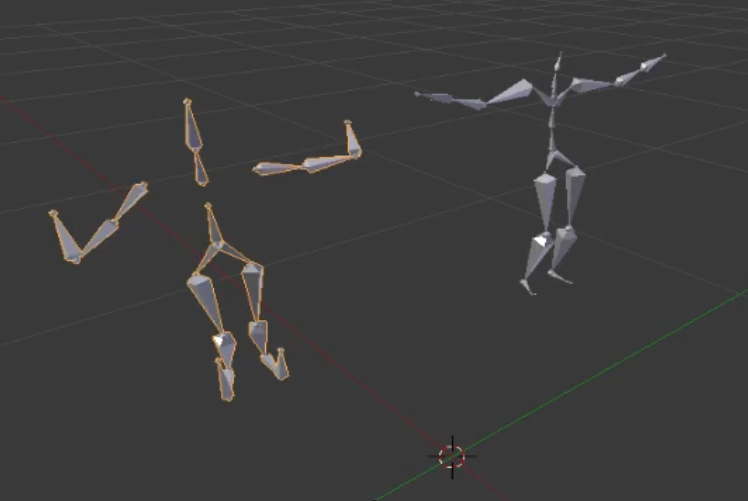
\includegraphics[width=1\linewidth, height=10cm]{images/retarget_wave.png}}
  \caption{Retargeted motion clip for skill of waving}
  \label{fig:retarget_wave}
\end{figure}
\begin{figure} 
  \centering
  \href{https://youtu.be/wdyNuvNhy3o}{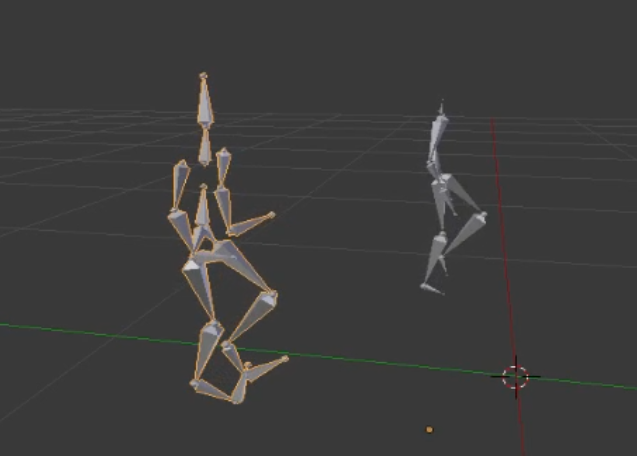
\includegraphics[width=1\linewidth, height=10cm]{images/retarget_wip.png}}
  \caption{Retargeted motion clip for walk in place skill}
  \label{fig:retarget_wip}
\end{figure}
\section{Training without Retargeting}
In the Training phase, initially to test the results of both phases independently we had manually created some motion clips which were free from retargeting errors. These include motion clips like hands opposite motion (in Fig \ref{fig:ho}), periodic squats motion (in Fig \ref{fig:squats}), manual partial walk in place motion (in Fig \ref{fig:mwip}). As you can see from these videos, that the robot is mimicking the motion to quite a good extent and further training will only improve these skills. All these skills have been trained using A3C code for around 50-60k episodes each using same reward function but with different state and action space. This space has been limited to only those joints that are changed in the motion clips (instead of all of the original 22 joints). 

\begin{figure}[!ht]
    \centering
    \subfloat[Hands Opposite Skill]{
    	\href{https://youtu.be/lfb5rWUCuvw}{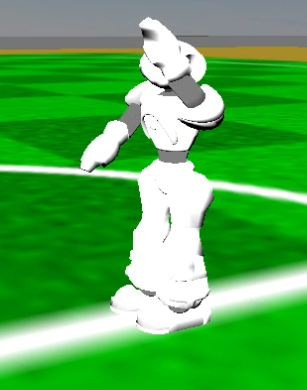
\includegraphics[width=0.3\linewidth, height=5cm,keepaspectratio]{images/ho.png}}
    	\label{fig:ho}
	}
    \qquad
    \subfloat[Squats Skill]{
    	\href{https://youtu.be/4LrHAHY2keg}{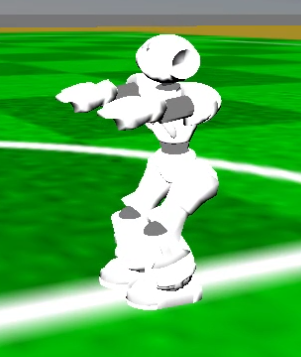
\includegraphics[width=0.3\linewidth, height=5cm,keepaspectratio]{images/squats.png}}
    	\label{fig:squats}
	}
    \qquad
    \subfloat[Walk in Place Skill]{
    	\href{https://youtu.be/yerCueG01oI}{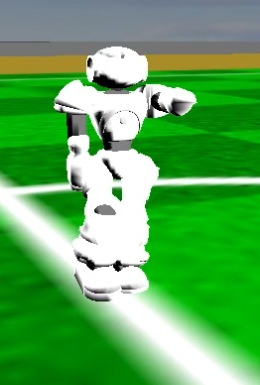
\includegraphics[width=0.3\linewidth, height=5cm,keepaspectratio]{images/mwip.png}}
    	\label{fig:mwip}
	}
    \label{fig:x1}
    \caption{Trained models for manually designed motion clips}
\end{figure}

\newpage
\section{Training with Retargeting}

After thorough testing, we also tried simulations over retargeted clips. These include hand wave motion (in Fig \ref{fig:wave}) and partial walk in place motion (in Fig \ref{fig:wip}). As you can see from the video of hand wave motion, that since the robot is well-balanced it can learn to mimic this motion quite well. However in case of walk in place motion, robot is not able to lift its leg as it has perhaps found a local minimum where lifting its leg only makes it fall (resulting in lower total reward) but partially copying the motion clip while maintaining balance gives higher cumulative reward. In this scenario, even though the retargeting seems smooth, learning to balance is a difficult task for our agent.

\begin{figure}[!ht]
    \centering
    \subfloat[Hand Wave Skill]{
    	\href{https://youtu.be/zeTAqHSJgxo}{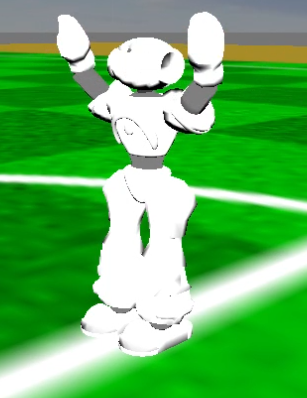
\includegraphics[width=0.4\linewidth, height=7cm]{images/wave.png}}
    	\label{fig:wave}
	}
    \qquad
    \subfloat[Walk in Place Skill]{
    	\href{https://youtu.be/IVX6FNjUJvo}{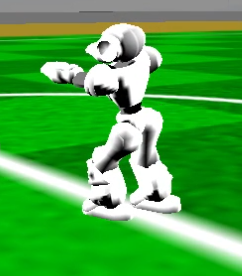
\includegraphics[width=0.4\linewidth, height=7cm]{images/wip.png}}
    	\label{fig:wip}
	}
    \qquad
    \label{fig:subfigname}
    \caption{Trained models for retargeted motion clips}
\end{figure}
